\documentclass{vkr}
\usepackage[english, russian]{babel} % переносы
\usepackage{graphicx} % для вставки картинок
\graphicspath{{images/}} % путь к изображениям
\usepackage[hidelinks]{hyperref}
\usepackage{float} % определяет метод H для рисунка с переносом на следующую страницу, ели не помещается
\usepackage{pdflscape}
\addto{\captionsrussian}{\renewcommand{\refname}{СПИСОК ИСПОЛЬЗОВАННЫХ ИСТОЧНИКОВ}}
\usepackage{xltabular} % для вставки таблиц
\usepackage{makecell}
\renewcommand\theadfont{} % шрифт в /thead
\usepackage{array} % для определения новых типов столбцов таблиц
\newcolumntype{T}{>{\centering\arraybackslash}X} % новый тип столбца T - автоматическая ширина столбца с выравниванием по центру
\newcolumntype{R}{>{\raggedleft\arraybackslash}X} % новый тип столбца R - автоматическая ширина столбца с выравниванием по правому краю
\newcolumntype{C}[1]{>{\centering\let\newline\\\arraybackslash\hspace{0pt}}m{#1}} % новый тип столбца C - фиксированная ширина столбца с выравниванием по центру
\newcolumntype{r}[1]{>{\raggedleft\arraybackslash}p{#1}} % новый тип столбца r - фиксированная ширина столбца с выравниванием по правому краю
\newcommand{\centrow}{\centering\arraybackslash} % командой \centrow можно центрировать одну ячейку (заголовок) в столбце типа X или p, оставив в оcтальных ячейках другой тип выравнивания
\newcommand{\finishhead}{\endhead\hline\endlastfoot}
\newcommand{\continuecaption}[1]{\captionsetup{labelformat=empty} \caption[]{#1}\\ \hline }
\usepackage{etoolbox}
\AtBeginEnvironment{xltabular}{\refstepcounter{tablecnt}} % подсчет таблиц xltabular, обычные таблицы подсчитываются в классе

\usepackage[tableposition=top]{caption} % подпись таблицы вверху
\captionsetup{strut=off}
\setlength{\intextsep}{0pt} % Vertical space above & below [h] floats
\setlength{\textfloatsep}{0pt} % Vertical space below (above) [t] ([b]) floats
\DeclareCaptionLabelFormat{gostfigure}{Рисунок #2} %подпись рисунка
\DeclareCaptionLabelFormat{gosttable}{Таблица #2} %подпись таблицы
\DeclareCaptionLabelSeparator{gost}{~--~} %разделитель в рисунках и таблицах
\captionsetup{labelsep=gost}
\captionsetup[figure]{aboveskip=10pt,belowskip=4mm,justification=centering,labelformat=gostfigure} % настройка подписи рисунка
\captionsetup[table]{font={stretch=1.41},skip=0pt,belowskip=0pt,aboveskip=8.5pt,singlelinecheck=off,labelformat=gosttable} % настройка подписи таблицы

\setlength{\LTpre}{8mm} % отступ сверху таблицы
\setlength{\LTpost}{6mm} % отступ снизу таблицы

\usepackage{enumitem}
\setlist{nolistsep,wide=\parindent,itemindent=*} % отступы вокруг списков, выравнивание с учетом разделителя

\usepackage{color} %% это для отображения цвета в коде
\usepackage{listings} %% листинги кода
\setmonofont[Scale=0.7]{Verdana} % моноширный шрифт для листинга

\definecolor{codegreen}{rgb}{0,0.6,0}
\definecolor{codegray}{rgb}{0.5,0.5,0.5}
\definecolor{codepurple}{rgb}{0.58,0,0.82}

\lstset{ %
language=C,                 % выбор языка для подсветки (здесь это С)
numbers=left,               % где поставить нумерацию строк (слева\справа)
numberstyle=\tiny,           % размер шрифта для номеров строк
stepnumber=1,                   % размер шага между двумя номерами строк
numbersep=5pt,                % как далеко отстоят номера строк от подсвечиваемого кода
commentstyle=\color{codegreen},
keywordstyle=\color{magenta},
numberstyle=\tiny\color{codegray},
stringstyle=\color{codepurple},
basicstyle=\linespread{0.95}\ttfamily,
backgroundcolor=\color{white}, % цвет фона подсветки - используем \usepackage{color}
showspaces=false,            % показывать или нет пробелы специальными отступами
showstringspaces=false,      % показывать или нет пробелы в строках
showtabs=false,             % показывать или нет табуляцию в строках
frame=single,              % рисовать рамку вокруг кода
tabsize=2,                 % размер табуляции по умолчанию равен 2 пробелам
captionpos=t,              % позиция заголовка вверху [t] или внизу [b] 
breaklines=true,           % автоматически переносить строки (да\нет)
breakatwhitespace=false, % переносить строки только если есть пробел
escapeinside={\%*}{*)}   % если нужно добавить комментарии в коде
}

\makeatletter % чтобы допускались русские комментарии в листингах
\lst@InputCatcodes
\def\lst@DefEC{%
 \lst@CCECUse \lst@ProcessLetter
  ^^80^^81^^82^^83^^84^^85^^86^^87^^88^^89^^8a^^8b^^8c^^8d^^8e^^8f%
  ^^90^^91^^92^^93^^94^^95^^96^^97^^98^^99^^9a^^9b^^9c^^9d^^9e^^9f%
  ^^a0^^a1^^a2^^a3^^a4^^a5^^a6^^a7^^a8^^a9^^aa^^ab^^ac^^ad^^ae^^af%
  ^^b0^^b1^^b2^^b3^^b4^^b5^^b6^^b7^^b8^^b9^^ba^^bb^^bc^^bd^^be^^bf%
  ^^c0^^c1^^c2^^c3^^c4^^c5^^c6^^c7^^c8^^c9^^ca^^cb^^cc^^cd^^ce^^cf%
  ^^d0^^d1^^d2^^d3^^d4^^d5^^d6^^d7^^d8^^d9^^da^^db^^dc^^dd^^de^^df%
  ^^e0^^e1^^e2^^e3^^e4^^e5^^e6^^e7^^e8^^e9^^ea^^eb^^ec^^ed^^ee^^ef%
  ^^f0^^f1^^f2^^f3^^f4^^f5^^f6^^f7^^f8^^f9^^fa^^fb^^fc^^fd^^fe^^ff%
  ^^^^20ac^^^^0153^^^^0152%
  % Basic Cyrillic alphabet coverage
  ^^^^0410^^^^0411^^^^0412^^^^0413^^^^0414^^^^0415^^^^0416^^^^0417%
  ^^^^0418^^^^0419^^^^041a^^^^041b^^^^041c^^^^041d^^^^041e^^^^041f%
  ^^^^0420^^^^0421^^^^0422^^^^0423^^^^0424^^^^0425^^^^0426^^^^0427%
  ^^^^0428^^^^0429^^^^042a^^^^042b^^^^042c^^^^042d^^^^042e^^^^042f%
  ^^^^0430^^^^0431^^^^0432^^^^0433^^^^0434^^^^0435^^^^0436^^^^0437%
  ^^^^0438^^^^0439^^^^043a^^^^043b^^^^043c^^^^043d^^^^043e^^^^043f%
  ^^^^0440^^^^0441^^^^0442^^^^0443^^^^0444^^^^0445^^^^0446^^^^0447%
  ^^^^0448^^^^0449^^^^044a^^^^044b^^^^044c^^^^044d^^^^044e^^^^044f%
  ^^^^0401^^^^0451%
  %%%
  ^^00}
\lst@RestoreCatcodes
\makeatother


% Режим шаблона (должен быть включен один из трех)

\Курсоваяtrue

\newcommand{\Дисциплина}{<<Проектирование и архитектура программных систем>>} % для курсовой
\newcommand{\КодСпециальности}{09.03.04} % Курсовая
\newcommand{\Специальность}{Программная инженерия} % Курсовая
\newcommand{\Тема}{Разработка web-сайта «Форум» на платформе} % ВКР Курсовая
\newcommand{\ТемаВтораяСтрока}{Python}
\newcommand{\ГдеПроводитсяПрактика}{Юго-Западном государственном университете} % для практики
\newcommand{\РуководительПрактПредпр}{Куркина А. В.} % для практики
\newcommand{\ДолжнРуководительПрактПредпр}{директор} % для практики
\newcommand{\РуководительПрактУнивер}{Чаплыгин А. А.} % для практики
\newcommand{\ДолжнРуководительПрактУнивер}{к.т.н. доцент} % для практики
\newcommand{\Автор}{Р. Д. Попов}
\newcommand{\АвторРод}{Попова Р.Д.}
\newcommand{\АвторПолностьюРод}{Попова Романа Денисовича} % для практики
\newcommand{\Шифр}{хх-хх-хххх}
\newcommand{\Курс}{4} % для практики
\newcommand{\Группа}{ПО-11б}
\newcommand{\Руководитель}{А. А. Чаплыгин} % для ВКР и курсовой
\newcommand{\Нормоконтроль}{А. А. Чаплыгин} % для ВКР
\newcommand{\ЗавКаф}{А. В. Малышев} % для ВКР
\newcommand{\ДатаПриказа}{«??» апреля 2023~г.} % для ВКР
\newcommand{\НомерПриказа}{1505-с} % для ВКР
\newcommand{\СрокПредоставления}{«??» июня 2023~г.} % для ВКР, курсового

\begin{document}
\maketitle
\ifПрактика{}\else{
   \newpage
\begin{center}
\large\textbf{Минобрнауки России}

\large\textbf{Юго-Западный государственный университет}
\vskip 1em
\normalsize{Кафедра программной инженерии}
\vskip 1em
\ifВКР{
        \begin{flushright}
        \begin{tabular}{p{.4\textwidth}}
        \centrow УТВЕРЖДАЮ: \\
        \centrow Заведующий кафедрой \\
        \hrulefill \\
        \setarstrut{\footnotesize}
        \centrow\footnotesize{(подпись, инициалы, фамилия)}\\
        \restorearstrut
        «\underline{\hspace{1cm}}»
        \underline{\hspace{3cm}}
        20\underline{\hspace{1cm}} г.\\
        \end{tabular}
        \end{flushright}
        }\fi
\end{center}
\vspace{1em}
  \begin{center}
  \large
\ifВКР{
ЗАДАНИЕ НА ВЫПУСКНУЮ КВАЛИФИКАЦИОННУЮ РАБОТУ
  ПО ПРОГРАММЕ БАКАЛАВРИАТА}
  \else
ЗАДАНИЕ НА КУРСОВУЮ РАБОТУ (ПРОЕКТ)
\fi
\normalsize
  \end{center}
\vspace{1em}
{\parindent0pt
  Студента \АвторРод, шифр\ \Шифр, группа \Группа
  
1. Тема «\Тема\ \ТемаВтораяСтрока»
\ifВКР{
утверждена приказом ректора ЮЗГУ от \ДатаПриказа\ № \НомерПриказа
}\fi.

2. Срок предоставления работы к защите \СрокПредоставления

3. Исходные данные для создания программной системы:

3.1. Перечень решаемых задач:}

\renewcommand\labelenumi{\theenumi)}

\begin{enumerate}
\item Исследовать актуальность создания форума в современном интернет-пространстве;
\item  Создание структуры базы данных для хранения тем, сообщений, пользовательских профилей и другой необходимой информации; 
\item разработка клиентской части с использованием HTML, CSS и JavaScript для создания динамичных и отзывчивых веб-страниц;
\item оценка эффективности выбранных технологий и методов решения задач;
\end{enumerate}

{\parindent0pt
  3.2. Входные данные и требуемые результаты для программы:}

\begin{enumerate}
\item Входными данными для программной системы являются: пользовательская информация, тема и сообщения, ПО.
\item Выходными данными для программной системы являются: ответы и комментарии; отображение профиля пользователя с его личной информацией; системные сообщения.
\end{enumerate}

{\parindent0pt

  4. Содержание работы (по разделам):
  
  4.1. Введение
  
  4.1. Анализ предметной области
  
4.2. Техническое задание: основание для разработки, назначение разработки,
требования к программной системе, требования к оформлению документации.

4.3. Технический проект: общие сведения о программной системе, проект
данных программной системы, проектирование архитектуры программной системы, проектирование пользовательского интерфейса программной системы.

4.4. Рабочий проект: спецификация компонентов и классов программной системы, тестирование программной системы, сборка компонентов программной системы.

4.5. Заключение

4.6. Список использованных источников

\списокПлакатов

\vskip 2em
\begin{tabular}{p{6.8cm}C{3.8cm}C{4.8cm}}
Руководитель \ifВКР{ВКР}\else работы (проекта) \fi & \lhrulefill{\fill} & \fillcenter\Руководитель\\
\setarstrut{\footnotesize}
& \footnotesize{(подпись, дата)} & \footnotesize{(инициалы, фамилия)}\\
\restorearstrut
Задание принял к исполнению & \lhrulefill{\fill} & \fillcenter\Автор\\
\setarstrut{\footnotesize}
& \footnotesize{(подпись, дата)} & \footnotesize{(инициалы, фамилия)}\\
\restorearstrut
\end{tabular}
}

\renewcommand\labelenumi{\theenumi.}

   \abstract{РЕФЕРАТ}

Объем работы равен \formbytotal{lastpage}{страниц}{е}{ам}{ам}. Работа содержит \formbytotal{figurecnt}{иллюстраци}{ю}{и}{й}, \formbytotal{tablecnt}{таблиц}{у}{ы}{}, \arabic{bibcount} библиографических источников и \formbytotal{числоПлакатов}{лист}{}{а}{ов} графического материала. Количество приложений – 2. Графический материал представлен в приложении А. Фрагменты исходного кода представлены в приложении Б.

Перечень ключевых слов: коммерческий сайт, Система, CMS, Битрикс, Joomla, аддитивные технологии, 3D-принтеры, услуги, сервисы, информатизация, автоматизация, информационные технологии, веб-форма,  Apache, классы, база данных, средства защиты информации, подсистема, компонент, модуль, сущность, информационный блок, метод, контент-редактор, администратор, пользователь, web-сайт.

Объектом разработки является веб-сайт форум на Python.

Целью выпускной квалификационной работы является исследование и оптимизация алгоритмов обработки запросов для обеспечения высокой производительности веб-сайта без применения фреймворков.

В процессе создания сайта были выделены основные сущности путем создания информационных блоков, использованы классы и методы модулей, обеспечивающие работу с сущностями предметной области, а также корректную работу web-сайта, разработаны разделы, содержащие информацию о компании, ее деятельности, производимой продукции и услугах, разработан сервис по заказу 3D-деталей.

При разработке сайта использовалась система управления контентом "<1С-Битрикс: Управление сайтом">.

Разработанный сайт был успешно внедрен в компании.

\selectlanguage{english}
\abstract{ABSTRACT}
  
The volume of work is \formbytotal{lastpage}{page}{}{s}{s}. The work contains \formbytotal{figurecnt}{illustration}{}{s}{s}, \formbytotal{tablecnt}{table}{}{s}{s}, \arabic{bibcount} bibliographic sources and \formbytotal{числоПлакатов}{sheet}{}{s}{s} of graphic material. The number of applications is 2. The graphic material is presented in annex A. The layout of the site, including the connection of components, is presented in annex B.

List of keywords: commercial website, System, CMS, Bitrix, Joomla, additive technologies, 3D printers, services, services, informatization, automation, information technology, web form, Apache, classes, database, component, module, entity, information block, method, content editor, administrator, user, web site.

The object of the research is the analysis of information technologies for the development of a production company's website.

The object of the development is the website of a company engaged in the production of 3D printers, the production of equipment for the creation of powders, software development and the organization of additive manufacturing centers.

The purpose of the final qualifying work is to attract customers, increase orders, inform about products and services by creating a company website.

In the process of creating the site, the main entities were identified by creating information blocks, classes and methods of modules were used to ensure work with the entities of the subject area, as well as the correct operation of the website, sections containing information about the company, its activities, products and services were developed, a service for ordering 3D parts was developed.

When developing the site, the content management system <<1C – Bitrix: Site Management>> was used.

The developed website was successfully implemented in the company.
\selectlanguage{russian}
}\fi
\tableofcontents
\section*{ОБОЗНАЧЕНИЯ И СОКРАЩЕНИЯ}

БД -- база данных.

ИС -- информационная система.

ИТ -- информационные технологии. 

КТС -- комплекс технических средств.

ОМТС -- отдел материально-технического снабжения. 

ПО -- программное обеспечение.

РП -- рабочий проект.

СУБД -- система управления базами данных.

ТЗ -- техническое задание.

ТП -- технический проект.

UML (Unified Modelling Language) -- язык графического описания для объектного моделирования в области разработки программного обеспечения.

\ifПрактика{}\else{\section*{ВВЕДЕНИЕ}
\addcontentsline{toc}{section}{ВВЕДЕНИЕ}

Аддитивные технологии (АТ) начали активно развиваться со времени получения первых трехмерных изображений изделий на дисплеях компьютеров. Начало положила стереолитография, затем довольно многочисленные новые принципы стали называть технологиями быстрого прототипирования, затем укоренилось название "<Аддитивные технологии">. Интенсивность развития данных технологий не имеет аналогов. АТ изменили процессы проектирования и конструирования изделий, превратив их в процессы непрерывного создания изделий. Современные проектирование и производство изделий невозможно представить без данного рода технологий. 3D-принтеры стали такими же распространенными, как и персональные компьютеры. С помощью 3D-принтеров получают ткани, обувь, продукты питания, а также выращивают человеческие органы. Во многих отраслях, например, в космической отрасли, альтернативы аддитивным технологиям нет.

АТ предполагают изготовление детали методом послойного нанесения материала, в отличие от традиционных методов формирования детали, за счёт удаления материала из массива заготовки.

При использовании АТ все стадии реализации проекта от идеи до материализации находятся в единой технологической цепи, в которой каждая технологическая операция выполняется в цифровой CAD/CAM/CAE-системе.

Современные компании, видя, как развиваются информационные технологии, пытаются использовать их выгодно для своего бизнеса, поэтому запускают свой web-сайт. С его помощью предприятие может заявить о себе, проинформировать потенциального заказчика об услугах или продуктах, которые предоставляет, а также позволяет пользователям сделать с помощью сайта онлайн-заказ, произвести покупку или оплатить счета.

Сайт считается лицом компании и может существенно повысить ее имидж. Любой пользователь сети Интернет сможет получить необходимую информацию о компании в любой момент, появляется возможность найти контактные телефоны, адрес и e-mail, чтобы связаться с компанией. Сейчас большинство клиентов узнают о ее существовании именно через сайт. Поэтому сайт можно назвать самой лучшей рекламой. 

Главной задачей профессионально построенного сайта является превращение посетителя, зашедшего на сайт, в потенциального клиента.

\emph{Цель настоящей работы} – разработка web-сайта компании для привлечения новой аудитории, увеличения заказов, рекламы продукции и услуг компании. Для достижения поставленной цели необходимо решить \emph{следующие задачи:}
\begin{itemize}
\item провести анализ предметной области;
\item разработать концептуальную модель web-сайта;
\item спроектировать web-сайт;
\item реализовать сайт средствами web-технологий.
\end{itemize}

\emph{Структура и объем работы.} Отчет состоит из введения, 4 разделов основной части, заключения, списка использованных источников, 2 приложений. Текст выпускной квалификационной работы равен \formbytotal{page}{страниц}{е}{ам}{ам}.

\emph{Во введении} сформулирована цель работы, поставлены задачи разработки, описана структура работы, приведено краткое содержание каждого из разделов.

\emph{В первом разделе} на стадии описания технической характеристики предметной области приводится сбор информации о деятельности компании, для которой осуществляется разработка сайта.

\emph{Во втором разделе} на стадии технического задания приводятся требования к разрабатываемому сайту.

\emph{В третьем разделе} на стадии технического проектирования представлены проектные решения для web-сайта.

\emph{В четвертом разделе} приводится список классов и их методов, использованных при разработке сайта, производится тестирование разработанного сайта.

В заключении излагаются основные результаты работы, полученные в ходе разработки.

В приложении А представлен графический материал.
В приложении Б представлены фрагменты исходного кода. 
}\fi
\section{Анализ предметной области}
\subsection{Характеристика предприятия и его деятельности. Тест длинного заголовка, не должен содержать переносы}

Технология трёхмерной печати появилась в конце 80-х гг. ХХ в. Пионером в этой области является компания 3D Systems, которая разработала первую коммерческую стереолитографическую машину – SLA – \linebreak Stereolithography Apparatus (1986 г.). До середины 90-х гг. она использовалась в научно-исследовательской и опытноконструкторской деятельности, связанной с оборонной промышленностью. Первые лазерные машины – сначала стереолитографические (SLA-машины), затем порошковые (SLS-машины) – были чрезмерно дороги, а выбор модельных материалов скромный. Широкое распространение цифровых технологий в области проектирования (CAD), моделирования и расчётов (CAE) и механообработки (CAM) стимулировало развитие технологий 3D-печати. 

Термин "<аддитивные технологии"> (АТ) означает изготовление изделия путем добавления. АТ являются новыми методами в производстве различного рода изделий. Применение данных технологий допускает как создание изделий с нуля, так и обработку уже имеющихся. Сегодня трудно найти отрасль производства, где бы ни применялись 3D-принтеры: с их помощью изготавливаются детали самолетов, космических аппаратов, подводных лодок, инструменты, протезы и др.

АТ предполагают изготовление (построение) физического объекта (детали) методом послойного нанесения материала, в отличие от традиционных методов формирования детали, за счёт удаления материала из массива заготовки.

АТ охватывают все новые сферы деятельности человека. Дизайнеры, архитекторы, кондитеры, археологи, астрономы, палеонтологи и представители других профессий используют 3D-принтеры для реализации различных идей и проектов. 

Деятельность отраслевого интегратора "<Русатом -- Аддитивные технологии"> охватывает все составляющие аддитивного рынка: производство 3D-принтеров, выпуск оборудования для создания порошков, разработка программного обеспечения и организация центров аддитивного производства. Сегодня аддитивные технологии внедряются в самые сложные и наукоемкие отрасли: атомную промышленность, аэрокосмическую индустрию, медицину, автомобилестроение и многие другие. Применение АТ решает задачи по снижению стоимости, сокращения срока изготовления изделий и обеспечение высокой персонализации деталей.
\subsection{Аддитивные технологии, их классификация}

Основное преимущество АТ состоит в том, что прототип создается за один прием, а исходными данными для него служит геометрическая модель детали. В итоге отпадает необходимость в планировании последовательности технологических процессов, специальном оборудовании для обработки материалов, транспортировке от станка к станку и т. д.

Экструзионная печать. Включает такие методы, как послойное наплавление и многоструйная печать.

Стереолитография. Стереолитографические принтеры используют специальные жидкие материалы, называемые "<фотополимерными смолами">.

Ламинирование. Слои материала наклеиваются друг на друга и обрезаются по контурам цифровой модели с помощью лазера или лезвия. 

\section{Техническое задание}
\subsection{Основание для разработки}

Основанием для разработки программного продукта служит задание по курсовой работе по дисциплине  "<Разработка web-форума \textquotedbl 8chan\textquotedbl\ на языке Python">.

\subsection{Цель и назначение разработки}

Основной задачей выпускной квалификационной работы является разработка web-форума.

Задачами данной разработки являются:
\begin{itemize}
\item создание разделов сайта с постами, профилём, постом непосредственно и главной страницы;
\item реализация формы для добавления постов и комментариев;
\item реализация формы для регистрации и авторизации;
\end{itemize}

\subsection{Требования пользователя к интерфейсу web-сайта}

Сайт должен включать в себя:
\begin{itemize}
    \item навигацию по темам;
    \item авторизацию и регистрацию;
    \item доступ для пользователя;
\end{itemize}

Композиция шаблона сайта представлена на рисунке ~\ref{templ:image}.

\begin{figure}[ht]
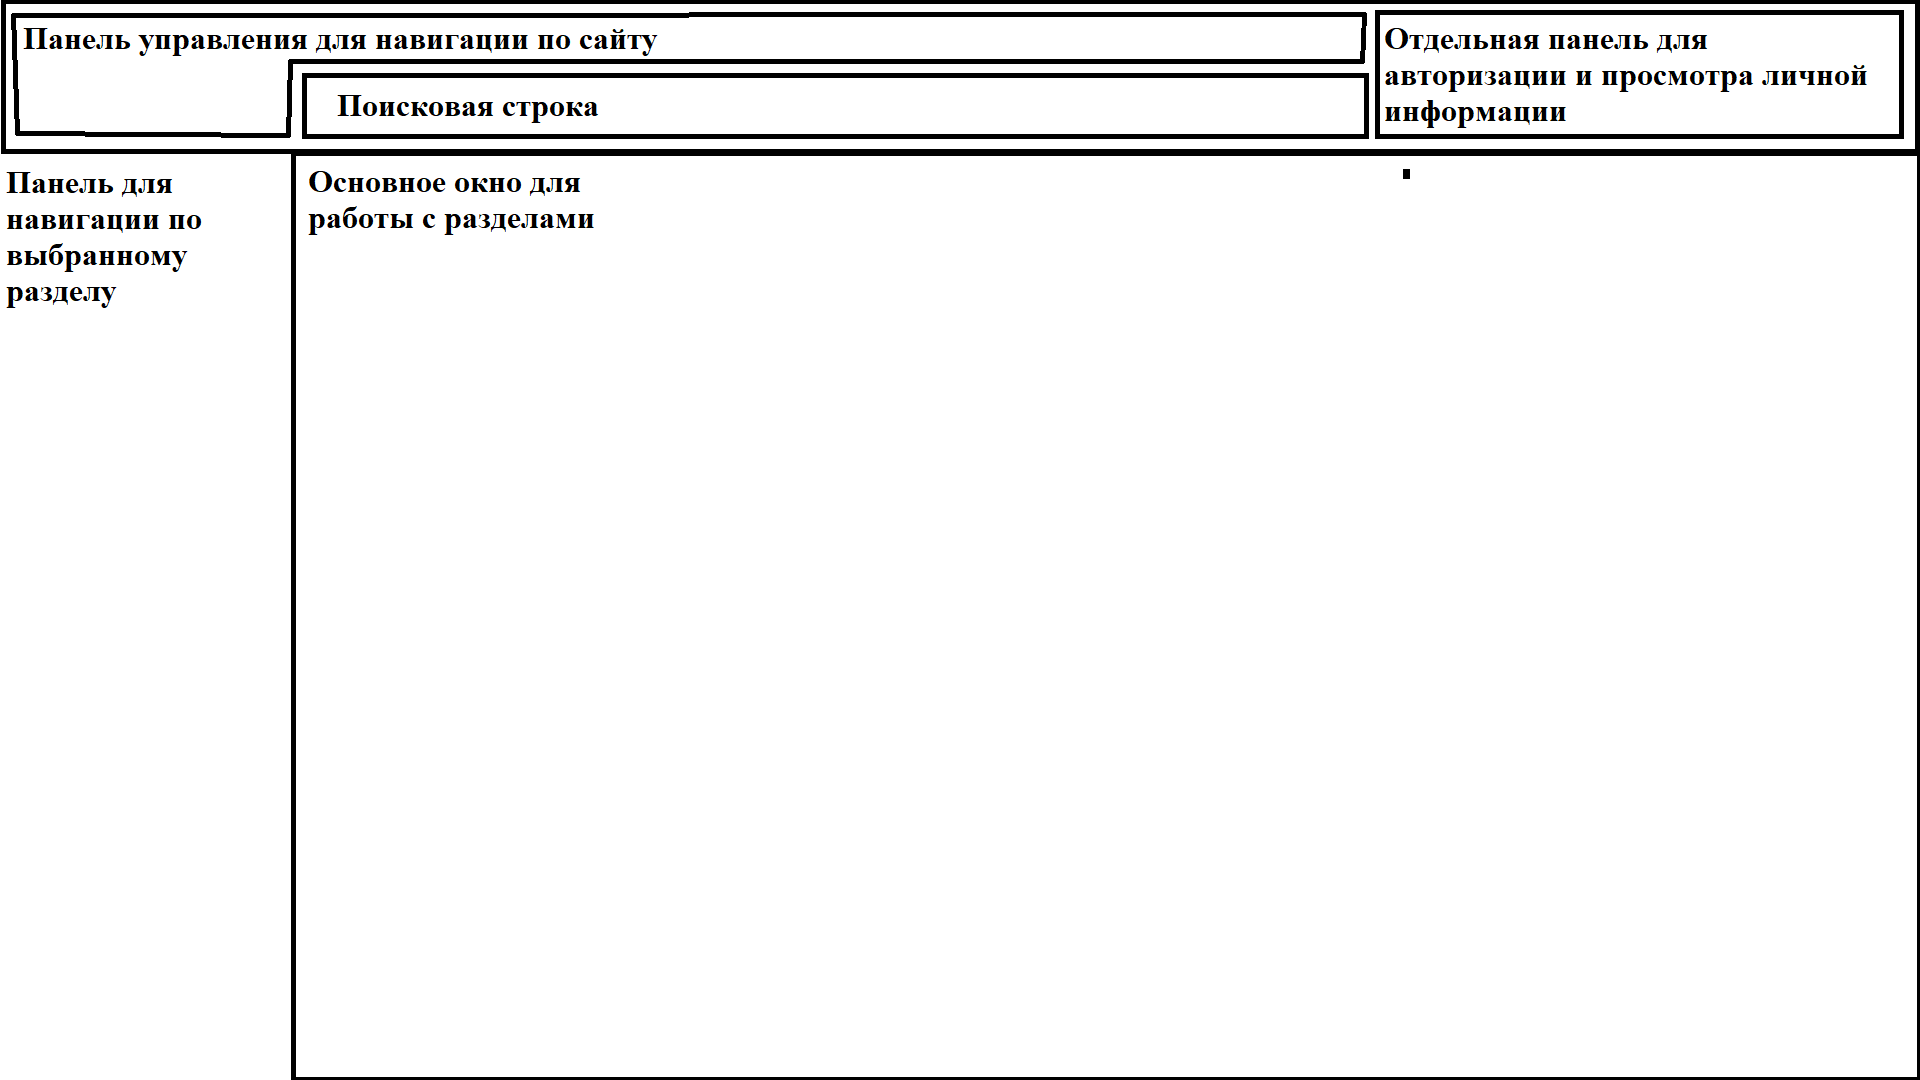
\includegraphics[width=1\linewidth]{templ}
\caption{Композиция шаблона сайта}
\label{templ:image}
\end{figure}
%\vspace{-\figureaboveskip} % двойной отступ не нужен (можно использовать, если раздел заканчивается картинкой)

\subsection{Моделирование вариантов использования}

Для разрабатываемого веб-сайта была создана модель, предоставляющая наглядное представление сценариев использования сайта. Эта модель является важным инструментом для физической разработки и подробного анализа взаимосвязей между объектами. При построении диаграммы вариантов использования используется унифицированный язык визуального моделирования (UML).

Диаграмма вариантов использования описывает функциональное предназначение разрабатываемой системы, представляя ее в виде ряда сценариев, предоставляемых системой актерам или сущностям, взаимодействующим с ней. Актерами являются внешние сущности, такие как пользователи или технические устройства, взаимодействующие с системой. Прецеденты описывают набор действий, предоставляемых системой актерам.

Таким образом, диаграмма вариантов использования служит начальным концептуальным представлением системы в процессе ее проектирования, представляя сценарии взаимодействия и действий, доступных пользователям и другим актерам.

На основании анализа предметной области в программе должны быть реализованы следующие прецеденты:
\begin{enumerate}
\item Регистрация нового пользователя
\item Авторизация пользователя
\item Добавление новой темы
\item Комментирование темы
\end{enumerate}

Диаграмма вариантов использования сайта представлена на рисунке 
~\ref{прецеденты:image}.

\begin{figure}[H]
	
	\center{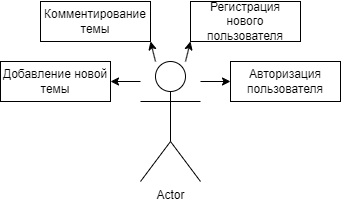
\includegraphics[width=0.7\linewidth]{прецеденты}}
	\caption{Прецеденты}
	\label{прецеденты:image}
\end{figure}

\subsubsection{Сценарии прецедентов программы}

\begin{enumerate}
	\item Сценарий для прецедента «Регистрация нового пользователя»:
	\begin{itemize}
		\item основной исполнитель: пользователь;
		\item заинтересованные лица и их требования: пользователю необходимо предоставить уникальный логин и пароль;
		\item предусловие: пользователь открыл веб-форум в браузере;
		\item основной успешный сценарий: пользователь вводит уникальный логин и пароль, система регистрирует нового пользователя.
	\end{itemize}
	\item Сценарий для прецедента «Авторизация пользователя»:
	\begin{itemize}
		\item основной исполнитель: пользователь;
		\item заинтересованные лица и их требования: пользователю необходимо предоставить зарегистрированный логин и пароль;
		\item предусловие: пользователь открыл веб-форум в браузере;
		\item основной успешный сценарий: пользователь вводит зарегистрированный логин и пароль, система производит авторизацию.
	\end{itemize}
	
	\item Сценарий для прецедента «Добавление новой темы»:
	\begin{itemize}
		\item основной исполнитель: пользователь;
		\item заинтересованные лица и их требования: пользователю необходимо написать заголовок темы и описание темы;
		\item предусловие: пользователь авторизован в системе;
		\item основной успешный сценарий: пользователь вводит заголовок темы и описание темы, добавляет её.
	\end{itemize}
	
	\item Сценарий для прецедента «Комментирование темы»:
	\begin{itemize}
		\item основной исполнитель: пользователь;
		\item заинтересованные лица и их требования: пользователю необходимо написать текст сообщения;
		\item предусловие: пользователь авторизован в системе;
		\item основной успешный сценарий: пользователь пишет текст сообщения, и отправляет его.
	\end{itemize}
	
\end{enumerate}

\subsection{Требования к оформлению документации}

Разработка программной документации и программного изделия должна производиться согласно ГОСТ 19.102-77 и ГОСТ 34.601-90. Единая система программной документации.

\section{Технический проект}
\subsection{Общая характеристика организации решения задачи}

Необходимо спроектировать и разработать сайт-форум для обсуждения на нём различных тем.


Веб-сайт — это комплекс взаимосвязанных электронных страниц, сгруппированных в разделы и доступных через уникальный интернет-адрес в форме www.имя\_сайта.ru. Каждая страница веб-сайта представляет собой текстовый документ, созданный с применением различных языков программирования, таких как HTML, CSS, JavaScript и другие.

\subsection{Обоснование выбора технологии проектирования}

На сегодняшний день информационный рынок, поставляющий программные решения в выбранной сфере, предлагает множество продуктов, позволяющих достигнуть поставленной цели – разработки web-сайта.

\subsubsection{Описание используемых технологий и языков программирования}

В процессе разработки web-сайта используются программные средства и языки программирования. Каждое программное средство и каждый язык программирования применяется для круга задач, при решении которых они необходимы.

\subsubsection{Язык программирования Python}

Python – это интерпретируемый, высокоуровневый язык программирования с динамической типизацией, который обеспечивает простоту в использовании, читаемость кода и эффективное взаимодействие с другими языками и системами. Основное предназначение данного языка – это создание серверной части веб-приложения, обеспечивая взаимодействие с веб-сервером. Это позволяет обрабатывать HTTP-запросы, управлять сессиями и осуществлять обработку данных от клиентов, а также взаимодействовать с базой данных.

\subsubsection{Язык программирования JavaScript}

\paragraph{Достоинства языка JavaScript}

JavaScript – это высокоуровневый, интерпретируемый язык программирования, который широко используется для создания интерактивных и динамичных веб-сайтов. Разработанный Netscape, JavaScript стал ключевым компонентом веб-технологий, позволяя веб-страницам взаимодействовать с пользователем, изменять содержимое и обеспечивать богатый пользовательский опыт. JavaScript используется для создания интерактивных элементов пользовательского интерфейса на веб-сайтах форумов. Это включает в себя динамическую подгрузку данных, анимации, обработку событий и обновление содержимого страницы без ее перезагрузки. JavaScript может обеспечивать валидацию данных, введенных пользователями в формах, перед отправкой на сервер. Также он применяется для асинхронного взаимодействия с сервером, например, для отправки комментариев, без необходимости перезагрузки всей страницы. JavaScript позволяет динамически обновлять содержимое форума в реальном времени. Это может включать в себя добавление новых тем, обновление сообщений, и другие изменения, которые пользователь может видеть без необходимости обновления всей страницы. JavaScript используется для взаимодействия с серверной частью, осуществляя запросы к API форума на Python. Это включает передачу данных между клиентом и сервером, а также обновление интерфейса в соответствии с полученными данными.

\paragraph{Недостатки языка Javascript}

JavaScript может вести себя по-разному в различных браузерах, что создает проблемы с кросс-браузерной совместимостью. Некоторые функции могут работать по-разному или вовсе отсутствовать в различных браузерах, что требует дополнительного тестирования и учета особенностей при разработке. JavaScript выполняется на стороне клиента, и поэтому пользователи могут иметь доступ к исходному коду и внести изменения. Это может создавать уязвимости безопасности, такие как внедрение вредоносного кода или модификация данных на стороне клиента. По соображениям безопасности JavaScript имеет ограниченный доступ к файловой системе клиентского устройства. Это может затруднить реализацию некоторых функций, таких как загрузка и сохранение файлов на стороне клиента. Средства отладки JavaScript в браузере могут быть менее мощными и удобными, чем средства отладки на сервере. Это может затруднить выявление и устранение ошибок в коде JavaScript. Обработка ошибок в JavaScript иногда может быть неочевидной из-за асинхронной природы языка. Это может затруднить выявление и отладку ошибок, особенно в сложных веб-приложениях.

\subsection{Диаграмма взаимодействия и схема обмена данными между представлениями}

Диаграмма взаимодействия описывает физическое представление системы и устанавливает связи между ее программными представлениями, включая исходный и исполняемый код. Она служит инструментом для определения архитектуры системы, выявляя зависимости между программными элементами. На диаграмме взаимодействия используются графические элементы, такие как представления, интерфейсы и их взаимосвязи.

Каждое представление должно быть активировано в контексте веб-страницы. В процессе вызова представления, данные передаются из веб-страницы в само представление.

Файл index.py представляет собой пример простого веб-приложения на Python, использующего фреймворк WSGI (Web Server Gateway Interface). В этом файле происходит импорт необходимых библиотек, классов и функций, таких как CGI, Waitress для веб-сервера, различные представления (views) и функции для работы с файлами и базой данных.



Словарь urls связывает URL-пути с соответствующими представлениями. Когда поступает запрос, код использует этот словарь для определения, какой обработчик использовать для конкретного URL. Основная функция app обрабатывает POST-запрос для загрузки файла, извлекает данные из формы, вставляет изображение в базу данных и возвращает ответ в формате JSON. Обработка GET-запроса осуществляется путем логики определения и вызова соответствующего представления, а также обработки статических файлов, установки MIME-типа и кодировки для ответа, установки заголовков ответа и возврата данных в ответе.


\subsubsection{Структура серверной части}
Структура серверной части мессенджера представлена следующим образом:

\begin{figure}[H]
	\centering
	\includegraphics[width=0.6\linewidth]{images/Server_diag}
	\caption{Диаграмма компонентов сервера}
	\label{fig:serverdiag}
\end{figure}

index.py - запускает веб-сервер Waitress, который обрабатывает HTTP-запросы с помощью функции маршрутизации route\_request. Он определяет приложение WSGI и запускает сервер для обработки входящих запросов и отправки ответов клиентам.

route\_request.py - обрабатывает входящие HTTP-запросы, сопоставляя их с маршрутами и вызывая соответствующие представления для генерации ответов. Он затем возвращает сгенерированные ответы клиенту, установив соответствующий код состояния и заголовки.

routes.py - определяет список маршрутов для веб-приложения, связывая URL-паттерны с соответствующими классами представлений. Он импортирует необходимые представления и указывает маршрут для обработки ошибок через ErrorView, который используется для всех несоответствующих URL.

templates\_view - определяют базовый класс View и различные классы представлений для обработки HTTP-запросов. Они реализуют методы для обработки GET и POST запросов, обрабатывают данные формы и взаимодействуют с базой данных, возвращая соответствующие ответы клиентам.

render\_template.py - определяет функцию render\_template, которая загружает HTML-шаблон из файла, подставляет в него данные из переданного словаря контекста и возвращает сгенерированный HTML-код в виде строки.

response.py - определяет класс Response, который формирует HTTP-ответы с заданными данными, типом контента и статусным кодом. Класс содержит методы для кодирования данных в UTF-8 и форматирования статусного кода с сообщением, обеспечивая удобное представление и передачу ответов в веб-приложении.

register.html и register.js - проверяет авторизацию пользователя через cookie и скрывает определенные элементы навигации для неавторизованных пользователей. Он также добавляет обработчик формы регистрации, который отправляет данные на сервер и обрабатывает ответ, перенаправляя пользователя на главную страницу при успешной регистрации.

login.html и login.js - для авторизации пользователей на веб-сайте. Он позволяет пользователям вводить свои учетные данные (логин и пароль) в форму, отправлять запрос на сервер для проверки этих данных среди зарегистрированных пользователей, и в случае успешной авторизации сохраняет информацию о пользователе в cookie и localStorage, что позволяет сайту опознавать пользователя и предоставлять доступ к защищенным ресурсам или персонализированным функциям.

app.js - играет ключевую роль в аутентификации пользователей, управлении интерфейсом навигации и обеспечении безопасного доступа к функциональности веб-приложения.


\subsubsection{Структура веб-клиента}
Структура веб-клиента мессенджера представлена следующим образом:

\begin{figure}[H]
	\centering
	\includegraphics[width=0.4\linewidth]{images/klient_diag}
	\caption{Диаграмма компонентов веб-клиента}
	\label{fig:klientdiag}
\end{figure}

\subsubsection{Диаграмма классов}
На рисунке \ref{fig:classdiag} изображена диаграмма классов для моего проекта веб-мессенджера. Данная диаграмма визуализирует взаимодействие между различными классами, представляющими пользователей, сообщения, чаты, элементы управления и другие основные компоненты системы.


\begin{figure}
	\centering
	\includegraphics[width=1.05\linewidth]{images/class_diag}
	\caption{Диаграмма классов}
	\label{fig:classdiag}
\end{figure}

TemplateView - эта группа классов представляет собой реализацию шаблонизации для веб-приложения. TemplateView служит базовым классом для создания видов, которые отображают содержимое HTML-шаблонов с данными из контекста.

View - этот базовый класс предоставляет общий интерфейс для обработки HTTP-запросов. Методы get и post позволяют переопределять поведение для обработки GET и POST запросов соответственно, а метод handle определяет, какой метод вызывать в зависимости от типа запроса (GET или POST), что делает его основой для создания различных видов (views) веб-приложения.

StaticView - этот класс-наследник View предназначен для обслуживания статических файлов веб-приложения. При получении GET запроса он открывает запрошенный файл из файловой системы, определяет MIME-тип и возвращает содержимое файла в виде HTTP-ответа с соответствующим кодом состояния (200 для успешного запроса или 404 в случае отсутствия файла).

CreateTopicView - этот класс-наследник TemplateView предназначен для обработки POST запросов при создании новой темы в форуме. При получении POST запроса извлекает данные формы, передает их в функцию create\_topic для сохранения в базе данных и возвращает успешный HTTP-ответ в формате JSON с кодом состояния 200.

CreateUserView - этот класс-наследник View обрабатывает POST запросы для создания нового пользователя. При получении POST запроса извлекает данные формы, передает их в функцию create\_user для регистрации пользователя в системе и возвращает успешный HTTP-ответ в формате JSON с кодом состояния 200.

GetMessagesView - этот класс-наследник View обрабатывает GET запросы для получения сообщений по указанной теме. При получении GET запроса извлекает параметры запроса, вызывает функцию get\_messages\_with\_username для извлечения данных из базы данных и возвращает полученные данные в формате JSON с кодом состояния 200.

GetTopicView - этот класс-наследник View обрабатывает GET запросы для получения списка тем из базы данных. При получении GET запроса вызывает функцию get\_topics\_from\_db для извлечения данных о темах и возвращает их в формате JSON с кодом состояния 200.

GetUsersView - этот класс-наследник View обрабатывает GET запросы для получения списка пользователей из базы данных. При получении GET запроса вызывает функцию get\_users\_from\_db для извлечения данных о пользователях и возвращает их в формате JSON с кодом состояния 200.

SendMessageView - этот класс-наследник View обрабатывает POST запросы для отправки сообщений в указанную тему. При получении POST запроса извлекает данные формы, передает их в функцию send\_message для сохранения сообщения в базе данных и возвращает успешный HTTP-ответ в формате JSON с кодом состояния 200.




\subsection{Содержание информационных блоков. Основные сущности}











Проанализировав требования, можно выделить три основных сущности:
\begin{itemize}
\item "<Пользователь">;
\item "<Сообщение">;
\item "<Тема">.
\end{itemize}

В состав сущности "<Сообщение"> можно включить атрибуты, представленные в таблице \ref{message:table}.

\begin{xltabular}{\textwidth}{|l|l|p{1.7cm}|X|}
	\caption{Атрибуты сущности "<Сообщение">\label{message:table}}\\ \hline
	\centrow Поле & \centrow Тип & \centrow Обяза\-тельное & \centrow Описание \\ \hline
	\thead{1} & \thead{2} & \centrow 3 & \centrow 4 \\ \hline
	\endfirsthead

	id\_message & Integer & true & Уникальный идентификатор сообщения \\ \hline 
	id\_user\_message & Integer & true & Уникальный идентификатор сообщения пользователя \\ \hline 
	topic\_id & Integer & true & Уникальный идентификатор темы, в которой написано сообщение \\ \hline 
	message\_text & String & true & Текст сообщения \\ \hline 
\end{xltabular}

В состав сущности "<Пользователь"> можно включить атрибуты, представленные в таблице \ref{user:table}.

\begin{xltabular}{\textwidth}{|l|lp{1.7cm}|X|}
	\caption{Атрибуты сущности "<Пользователь">\label{user:table}}\\ \hline
	\centrow Поле & \centrow Тип & \centrow Обяза\-тельное & \centrow Описание \\ \hline
	\thead{1} & \thead{2} & \centrow 3 & \centrow 4 \\ \hline
	\endfirsthead
	id\_user & Integer & true & Уникальный идентификатор пользователя \\ \hline 
	login & String & true & Имя пользователя \\ \hline 
	password & String & true & Пароль пользователя \\ \hline 
\end{xltabular}

В состав сущности "<Тема"> можно включить атрибуты, представленные в таблице \ref{topic:table}.

\begin{xltabular}{\textwidth}{|l|l|p{1.7cm}|X|}
	\caption{Атрибуты сущности "<Тема">\label{topic:table}}\\ \hline
	\centrow Поле & \centrow Тип & \centrow Обяза\-тельное & \centrow Описание \\ \hline
	\thead{1} & \thead{2} & \centrow 3 & \centrow 4 \\ \hline
	\endfirsthead
	id\_message & Integer & true & Уникальный идентификатор сообщения \\ \hline 
	id\_user\_message & Integer & true & Уникальный идентификатор сообщения пользователя \\ \hline 
	topic\_id & Integer & true & Уникальный идентификатор темы, в которой написано сообщение \\ \hline 
	message\_text & String & true & Текст сообщения \\ \hline 
\end{xltabular} 

\ifПрактика{}\else{
   \section{Рабочий проект}
\subsection{Классы, используемые при разработке сайта}

Можно выделить следующий список классов и их методов, использованных при разработке web-приложения (таблица \ref{class:table}).

\renewcommand{\arraystretch}{0.8} % уменьшение расстояний до сетки таблицы
\begin{xltabular}{\textwidth}{|X|p{2.5cm}|>{\setlength{\baselineskip}{0.7\baselineskip}}p{4.85cm}|>{\setlength{\baselineskip}{0.7\baselineskip}}p{4.85cm}|}
\caption{Описание классов View, используемых в приложении\label{class:table}}\\
\hline \centrow \setlength{\baselineskip}{0.7\baselineskip} Название класса & \centrow \setlength{\baselineskip}{0.7\baselineskip} Модуль, к которому относится класс & \centrow Описание класса & \centrow Методы \\
\hline \centrow 1 & \centrow 2 & \centrow 3 & \centrow 4\\ \hline
\endfirsthead
\caption*{Продолжение таблицы \ref{class:table}}\\
\hline \centrow 1 & \centrow 2 & \centrow 3 & \centrow 4\\ \hline
\finishhead
View & Главный модуль & View – основной класс для взаимодействия сервера с веб-страницами. Абстрактный класс, от которого наследуются все остальные view-классы. & template = '' – переменная для шаблонов дочерних классов.
def get(self, environ) – метод обработки GET-запросов.
def post(self, environ) – метод обработки POST-запросов.
def handle(self, environ) – метод для определения типа запроса (GET или POST) и вызова соответствующего метода.  \\
\hline CreateTopicView & Главный модуль & CreateTopicView – класс для обработки страницы создания темы. & template = 'templates/create_topic.html' – путь к HTML шаблону.
def post(self, environ) – метод для обработки формы создания темы и сохранения данных в базе данных. Возвращает JSON ответ о статусе операции.  \\

\hline ErrorView & Главный модуль & ErrorView – класс для обработки страницы ошибок. & template = template = 'templates/404.html' – путь к HTML шаблону для страницы ошибки.  \\


\hline GetMessagesView & Главный модуль & GetMessagesView – класс для получения сообщений с сервера. & def get(self, environ) – метод для обработки GET-запроса, получения сообщений из базы данных и возврата их в формате JSON.  \\

\hline IndexView & Главный модуль & IndexView – класс для отображения главной страницы. & template = 'templates/index.html' – путь к HTML шаблону главной страницы.  \\

\hline GetTopicView & Главный модуль & GetTopicView – класс для получения списка тем с сервера. & def get(self, environ) – метод для обработки GET-запроса, получения списка тем из базы данных и возврата их в формате JSON.  \\

\hline GetUsersView & Главный модуль & GetUsersView – класс для получения списка пользователей с сервера. & def get(self, environ) – метод для обработки GET-запроса, получения списка пользователей из базы данных и возврата их в формате JSON.  \\


\hline RegisterView & Главный модуль & RegisterView – класс для обработки страницы регистрации. & template = 'templates/register.html' – путь к HTML шаблону страницы регистрации. \\

\hline SendMessageView & Главный модуль & SendMessageView – класс для обработки отправки сообщений. & def post(self, environ) – метод для обработки формы отправки сообщений и сохранения данных в базе данных. Возвращает JSON ответ о статусе операции.   \\

\hline StaticView & Главный модуль & StaticView – класс для обработки статических файлов. & def get(self, environ) – метод для получения статического файла по запросу и возврата его содержимого с соответствующим MIME-типом.   \\

\hline TemplateView & Главный модуль & TemplateView – абстрактный класс для обработки страниц с HTML шаблонами. & template = '' – переменная для пути к HTML шаблону. def get(self, environ) – метод для рендеринга HTML шаблона и возврата его содержимого.   \\


\hline TopicPageView & Главный модуль & TopicPageView – класс для отображения страницы конкретной темы. & template = 'templates/topic_page.html' – путь к HTML шаблону страницы темы. \\



\hline TopicsView & Главный модуль & TopicsView – класс для отображения страницы со списком тем. & template = 'templates/topics.html' – путь к HTML шаблону страницы со списком тем. \\

\hline UserView & Главный модуль & UserView – класс для отображения страницы профиля пользователя. & template = 'templates/user.html' – путь к HTML шаблону страницы профиля.  \\

\end{xltabular}
\renewcommand{\arraystretch}{1.0} % восстановление сетки

\newpage
\subsection{Системное тестирование разработанного web-сайта}

На рисунке \ref{main:image} представлена главная страница сайта форума «8chan».

\begin{figure}[H] % H - рисунок обязательно здесь, или переносится, оставляя пустоту
\center{\includegraphics[width=1\linewidth]{main1}}
\caption{Главная страница сайта «8chan»}
\label{main:image}
\end{figure}

На рисунке \ref{menu:image} представлен динамический вывод тем.

\begin{figure}[ht]
\center{\includegraphics[width=1\linewidth]{menu}}
\caption{Динамический вывод тем}
\label{menu:image}
\end{figure}

На рисунке \ref{enter:image} представлен ввод данных для публикации темы.

\begin{figure}[ht]
\center{\includegraphics[width=1\linewidth]{enter}}
\caption{Ввод данных для публикации темы}
\label{enter:image}
\end{figure}

   \section*{ЗАКЛЮЧЕНИЕ}
\addcontentsline{toc}{section}{ЗАКЛЮЧЕНИЕ}

В условиях активного развития информационных технологий многие компании стремятся использовать веб-сайты для продвижения своего бизнеса. В рамках данного исследования был разработан веб-сайт для форума "8chan" с использованием языка программирования Python без применения фреймворков.

Основные результаты работы:

\begin{enumerate}
\item Анализ предметной области, выявление требований и необходимость выбора дополнительных языков для реализации.
\item Разработана концептуальная модель web-сайта. Разработана модель данных системы. Определены требования к системе.
\item Осуществлено проектирование web-сайта. Разработана архитектура серверной части. Разработан пользовательский интерфейс web-сайта.
\item Реализован и протестирован web-сайт. Проведено системное тестирование.
\end{enumerate}

Все требования, объявленные в техническом задании, были полностью реализованы, все задачи, поставленные в начале разработки проекта, были также решены.

Готовый рабочий проект представлен адаптивной версткой сайта.

}\fi
\addcontentsline{toc}{section}{СПИСОК ИСПОЛЬЗОВАННЫХ ИСТОЧНИКОВ}

\begin{thebibliography}{9}

    \bibitem{javascript} Фримен, А. Практикум по программированию на JavaScript / А. Фримен. – Москва~: Вильямс, 2013. – 960 с. – ISBN 978-5-8459-1799-7. – Текст~: непосредственный.
    \bibitem{php} Бретт, М. PHP и MySQL. Исчерпывающее руководство / М. Бретт. – Санкт-Петербург : Питер, 2016. – 544 с. – ISBN 978-5-496-01049-8. – Текст~: непосредственный.
    \bibitem{css} Веру, Л. Секреты CSS. Идеальные решения ежедневных задач / Л. Веру. – Санкт-Петербург : Питер, 2016. – 336 с. – ISBN 978-5-496-02082-4. – Текст~: непосредственный.
    \bibitem{mysql}	Гизберт, Д. PHP и MySQL / Д. Гизберт. – Москва~: НТ Пресс, 2013. – 320 с. – ISBN 978-5-477-01174-2. – Текст~: непосредственный.
	\bibitem{html5}	Голдстайн, А. HTML5 и CSS3 для всех / А. Голдстайн, Л. Лазарис, Э. Уэйл. – Москва~: Вильямс, 2012. – 368 с. – ISBN 978-5-699-57580-0. – Текст~: непосредственный.
	\bibitem{htmlcss}	Дэкетт, Д. HTML и CSS. Разработка и создание веб-сайтов / Д. Дэкетт. – Москва~: Эксмо, 2014. – 480 с. – ISBN 978-5-699-64193-2. – Текст~: непосредственный.
	\bibitem{bigbook}	Макфарланд, Д. Большая книга CSS / Д. Макфарланд. – Санкт-Петербург : Питер, 2012. – 560 с. – ISBN 978-5-496-02080-0. – Текст~: непосредственный.
	\bibitem{uchiru}	Лоусон, Б. Изучаем HTML5. Библиотека специалиста / Б. Лоусон, Р. Шарп. – Санкт-Петербург : Питер, 2013 – 286 с. – ISBN 978-5-459-01156-2. – Текст~: непосредственный.
	\bibitem{chaynik}	Титтел, Э. HTML5 и CSS3 для чайников / Э. Титтел, К. Минник. – Москва~: Вильямс, 2016 – 400 с. – ISBN 978-1-118-65720-1. – Текст~: непосредственный.    
	\bibitem{22}	Титтел, Э. HTML5 и CSS3 для чайников / Э. Титтел, К. Минник. – Москва~: Вильямс, 2016 – 400 с. – ISBN 978-1-118-65720-1. – Текст~: непосредственный.    
	\bibitem{1231}	Титтел, Э. HTML5 и CSS3 для чайников / Э. Титтел, К. Минник. – Москва~: Вильямс, 2016 – 400 с. – ISBN 978-1-118-65720-1. – Текст~: непосредственный.    
	\bibitem{sdf}	Титтел, Э. HTML5 и CSS3 для чайников / Э. Титтел, К. Минник. – Москва~: Вильямс, 2016 – 400 с. – ISBN 978-1-118-65720-1. – Текст~: непосредственный.    
	\bibitem{servsssds}	Титтел, Э. HTML5 и CSS3 для чайников / Э. Титтел, К. Минник. – Москва~: Вильямс, 2016 – 400 с. – ISBN 978-1-118-65720-1. – Текст~: непосредственный.
\end{thebibliography}

\ifВКР{\appendix{Представление графического материала}

Графический материал, выполненный на отдельных листах,
изображен на рисунках А.1--А.\arabic{числоПлакатов}.
\setcounter{числоПлакатов}{0}

\renewcommand{\thefigure}{А.\arabic{figure}} % шаблон номера для плакатов

\begin{landscape}

\begin{плакат}
    
\includegraphics[width=0.82\linewidth]{плакат1.png}
    \заголовок{Сведения о ВКРБ}
    \label{pl1:image}      
\end{плакат}

\begin{плакат}
    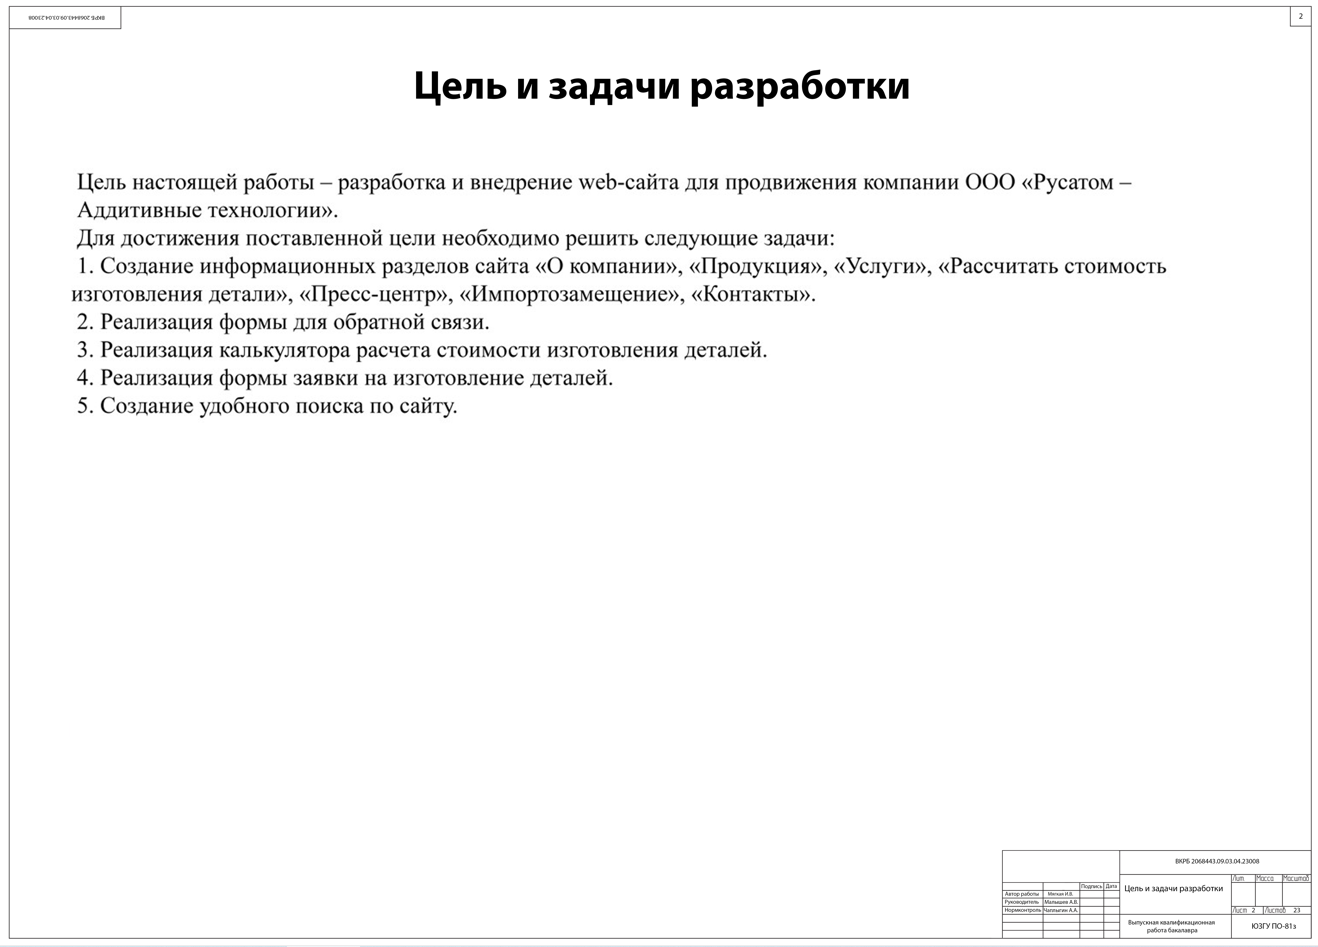
\includegraphics[width=0.82\linewidth]{плакат2.png}
    \заголовок{Цель и задачи разработки}
    \label{pl2:image}      
\end{плакат}

\begin{плакат}
    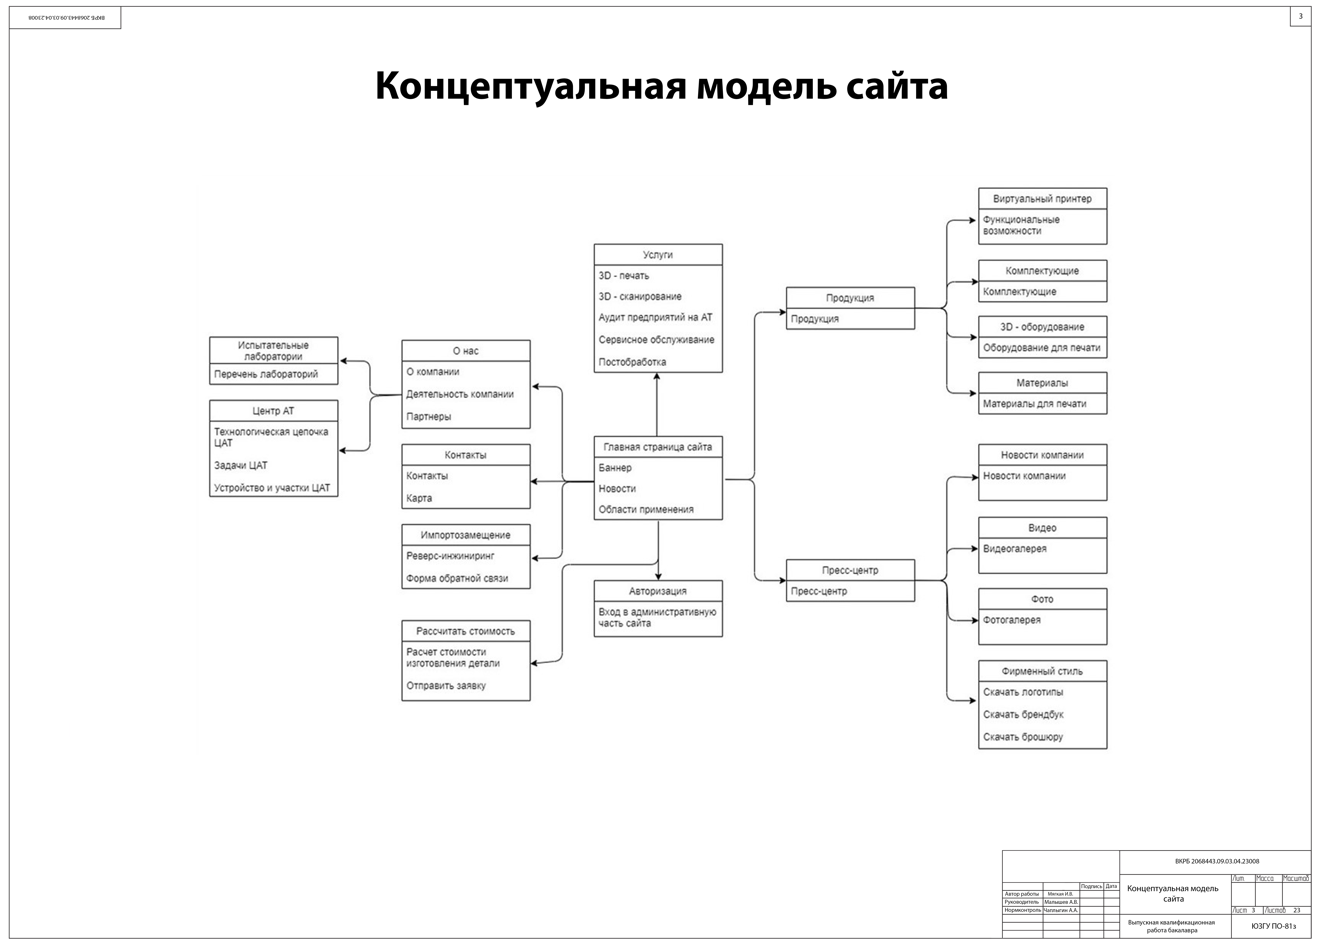
\includegraphics[width=0.82\linewidth]{плакат3.png}
    \заголовок{Концептуальная модель сайта}
    \label{pl3:image}      
\end{плакат}

\begin{плакат}
    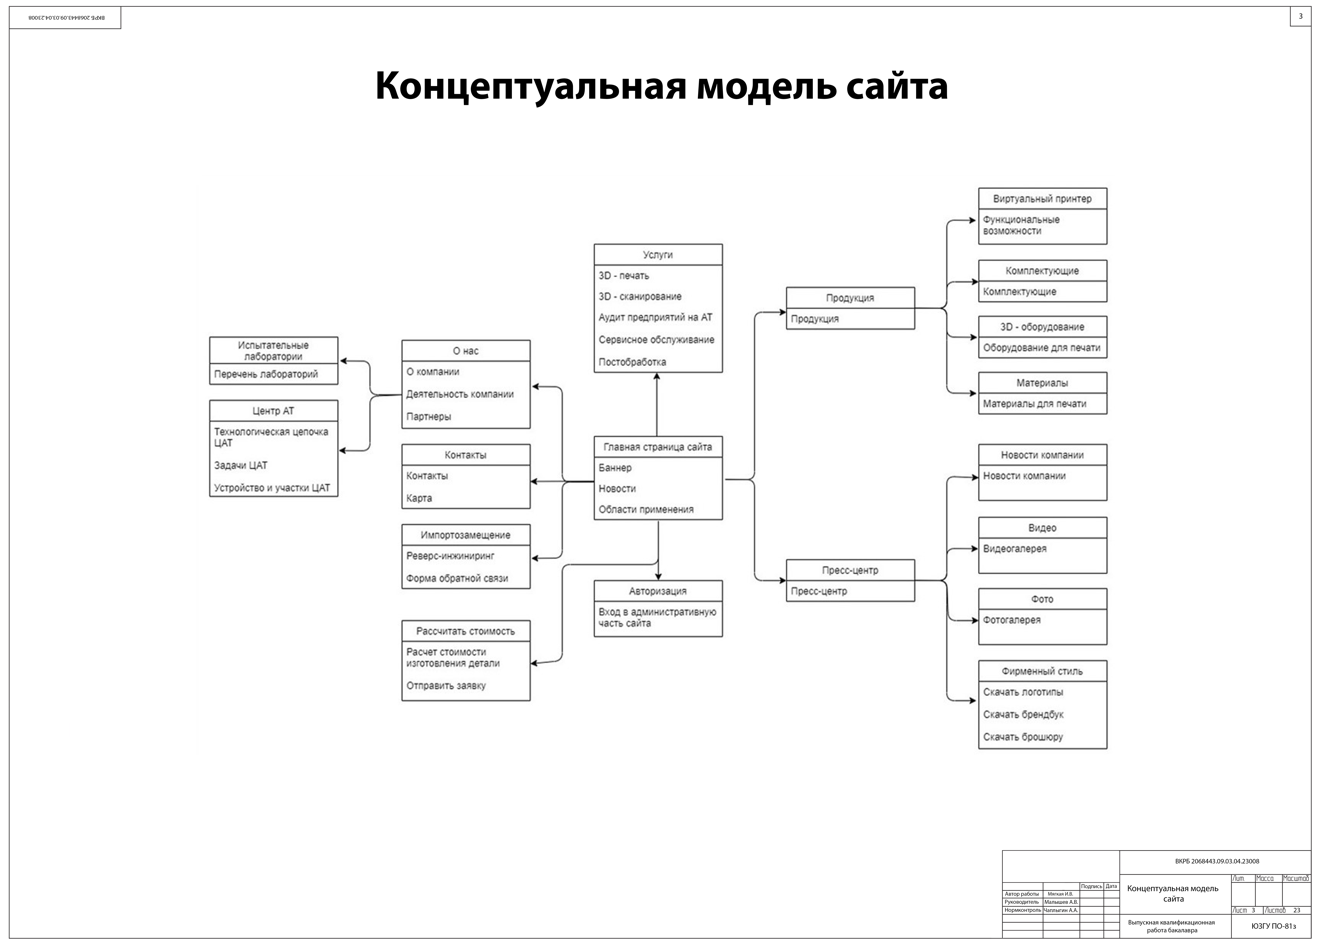
\includegraphics[width=0.82\linewidth]{плакат3.png}
    \заголовок{Еще плакат}
    \label{pl4:image}      
\end{плакат}

\end{landscape}
}\fi
\ifПрактика{}\else{\appendix{Фрагменты исходного кода программы}


codes.py
\lstinputlisting[language=Python, frame=none]{code/codes.py}

response.py
\lstinputlisting[language=Python, frame=none]{code/response.py}

routes.py
\lstinputlisting[language=Python, frame=none]{code/routes.py}

index.py
\lstinputlisting[language=Python, frame=none]{code/index.py}

index.py
\lstinputlisting[language=Python, frame=none]{code/index.py}

render\_template.py
\lstinputlisting[language=Python, frame=none]{code/render_template.py}

base\_view.py
\lstinputlisting[language=Python, frame=none]{code/base_view.py}

index\_view.py
\lstinputlisting[language=Python, frame=none]{code/index_view.py}

create\_topic\_view.py
\lstinputlisting[language=Python, frame=none]{code/create_topic_view.py}

get\_topic\_view.py
\lstinputlisting[language=Python, frame=none]{code/get_topic_view.py}

get\_users\_view.py
\lstinputlisting[language=Python, frame=none]{code/get_users_view.py}

register\_view.py
\lstinputlisting[language=Python, frame=none]{code/register_view.py}

static\_view.py
\lstinputlisting[language=Python, frame=none]{code/static_view.py}

topic\_page\_view.py
\lstinputlisting[language=Python, frame=none]{code/topic_page_view.py}

topics\_view.py
\lstinputlisting[language=Python, frame=none]{code/topics_view.py}

user.py
\lstinputlisting[language=Python, frame=none]{code/user.py}

}\fi
\end{document}
